\chapter{The Integral: Accumulation of a Rate Function}
\label{ch:integrals}

The previous few chapters dealt with differential calculus, which revolved around the concept of the rate of change of a function. We started with the simple geometric idea of the slope of a tangent line to a curve, developed it into a combination of theory about derivatives and their properties, techniques for calculating derivatives, and applications of derivatives. This chapter deals with integral calculus and starts with the simple geometric idea of area and relates it to the accumulation of a rate function. This idea will be developed into another combination of theory, techniques, and applications.

%\section{Accumulation}
\label{sec:accumulation}
% From Section 3.1

\subsection{Accumulation in Real Life}
We have already seen that the area under a graph can represent quantities whose units are not the usual geometric units of square meters or square feet. For example, if $t$ is a measure of time in seconds and $f(t)$ is a velocity with units of feet/second, then the definite integral has units (feet/second)$\cdot$(seconds) $=$ feet.

In general, the units for the definite integral $\int_a^bf(x)\,dx$ are ($y$-units)$\cdot$($x$-units). A quick check of the units can help avoid errors in setting up an applied problem.

In previous examples, we looked at a function that represented a rate of travel (miles per hour); in that case, the area represented the total distance traveled. For functions representing other rates such as the production of a factory (bicycles per day), or the flow of water in a river (gallons per minute) or traffic over a bridge (cars per minute), or the spread of a disease (newly sick people per week), the area will still represent the total amount of something.

\begin{example}
Suppose $MR(q)$ is the marginal revenue in dollars/item for selling $q$ items. What does $\int_0^{150}MR(q)\,dq$ represent?

\begin{solution}
  $\int_0^{150}MR(q)\,dq$ has units (dollars/item)$\cdot$(items) $=$ dollars, and represents the accumulated dollars for selling from 0 to 150 items. That is, $\int_0^{150}MR(q)\,dq=TR(150)$, the total revenue from selling 150 items.
\end{solution}\end{example}

\begin{example}
Suppose $r(t)$ represents the rate of change of the diameter of a tree, in centimeters per year. What does $\int_{T_1}^{T_2}r(t)\,dt$ represent?

\begin{solution}
  $\int_{T_1}^{T_2}r(t)\,dt$ has units of (centimeters per year)$\cdot$(years) $=$ centimeters, and represents the accumulated growth of the tree's diameter from time $T_1$ years to $T_2$ years. That is, $\int_{T_1}^{T_2}r(t)\,dt$ is the change in the diameter of the tree over this period of time.
\end{solution}\end{example}

\section{Approximating Area}
\label{sec:area-approx}
% From Section 3.1.
\subsection{PreCalculus Idea – The Area of a Rectangle}
If you look on the inside cover of nearly any traditional math book, you will find a bunch of area and volume formulas – the area of a square, the area of a trapezoid, the volume of a right circular cone, and so on. Some of these formulas are pretty complicated. But you still won't find a formula for the area of a jigsaw puzzle piece or the volume of an egg. There are lots of things for which there is no formula. Yet we might still want to find their areas.

One reason areas are so useful is that they can represent quantities other than simple geometric shapes. If the units for each side of the rectangle are meters, then the area will have the units meters$\times$meters = square meters = m$^2$. But if the units of the base of a rectangle are hours and the units of the height are miles/hour, then the units of the area of the rectangle are hours$\times$miles/hour = miles, a measure of distance. Similarly, if the base units are centimeters and the height units are grams, then the area units are gram-centimeters, a measure of work.

\begin{figure}[!ht]
  \centering
    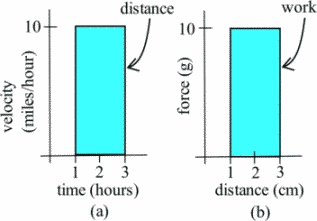
\includegraphics[width=0.4\textwidth]{img/chap5/image065.png}
    \caption{Modeling distance traveled and work with rectangles}
    \label{fig:5-2-rectangles}
\end{figure}
The basic shape we will use is the rectangle; the area of a rectangle is base$\times$height. You should also know the area formulas for triangles: $A=\dfrac{1}{2}bh$, and for circles: $A=\pi r^2$.

%Section 3.1: The Definite Integral
\subsection{Distance from Velocity}
\begin{example}
Suppose a car travels on a straight road at a constant speed of 40 miles per hour for two hours. See the graph of its velocity in Figure \ref{fig:5-2-distance}. How far has it gone?

\begin{figure}[!ht]
  \centering
    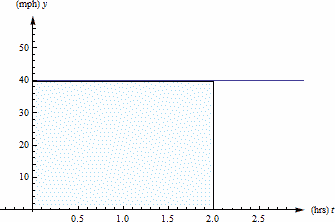
\includegraphics[width=0.4\textwidth]{img/chap5/image001.png}
    \caption{Car velocity as a function of time.}
    \label{fig:5-2-distance}
\end{figure}
\begin{solution}
We all remember distance = rate$\times$time, so this one is easy. The car has gone (40 miles/hour)$\times$(2 hours) = 80 miles.
\end{solution}\end{example}

\begin{example}
Now suppose that a car travels so that its speed increases steadily from 0 to 40 miles per hour, for two hours. (Just be grateful you weren’t stuck behind this car on the highway.) See the graph of its velocity in below. How far has this car gone?

\begin{figure}[!ht]
  \centering
    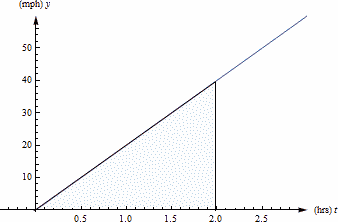
\includegraphics[width=0.4\textwidth]{img/chap5/image002.png}
    \caption{Car velocity as a function of time.}
    \label{fig:5-2-distance2}
\end{figure}

\begin{solution}
The trouble with our old reliable distance = rate$\times$time relationship is that it only works if the rate is constant. If the rate is changing, there isn’t a good way to use this formula.

But look at the graph from the last example again. Notice that distance = rate$\times$time also describes the area between the velocity graph and the $t$-axis, between $t=0$ and $t=2$ hours. The rate is the height of the rectangle, the time is the length of the rectangle, and the distance is the area of the rectangle. This is the way we can extend our simple formula to handle more complicated velocities: And this is the way we can answer the second example.

The distance the car travels is the area between its velocity graph, the $t$-axis, $t=0$ and $t=2$. This region is a triangle, so its area is
$$\frac{1}{2}bh = \frac{1}{2}(2 \text{ hours})(40 \text{ miles per hour}) = 40 \text{ miles}\enspace .$$
So the car travels 40 miles during its annoying trip.
\end{solution}\end{example}

In our distance/velocity examples, the function represented a rate of travel (miles per hour), and the area represented the total distance traveled. This principle works more generally.

For functions representing other rates such as the production of a factory (bicycles per day), or the flow of water in a river (gallons per minute) or traffic over a bridge (cars per minute), or the spread of a disease (newly sick people per week), the area will still represent the total amount of something.

graph
\begin{example}
The graph below shows the flow rate (cubic feet per second) of water in the Skykomish river at the town of Goldbar in Washington state.

graph
\begin{solution}
The area of the shaded region represents the total volume (cubic feet or ft$^3$) of water flowing past the town during the month of October. We can approximate this area to approximate the total water by thinking of the shaded region as a rectangle with a triangle on top.
\begin{align*}
\text{Total water} &= \text{total area} \\
  &\approx \text{area of rectangle} + \text{area of the ``triangle''}\\
  &\approx  \left(2000 \frac{\text{ft}^3}{\text{s}}\right)(30 \text{days})+12\left(1500\frac{\text{ft}^3}{\text{s}}\right)(30 \text{days})\\
  &= \left(2570 \frac{\text{ft}^3}{\text{s}}\right)(30 \text{days})
\end{align*}
Note that we need to convert the units to make sense of our result:
\begin{align*}
\text{Total water} &\approx  \left(2570 \frac{\text{ft}^3}{\text{s}}\right)(30 \text{days}) \\
  &=\left(2570 \frac{\text{ft}^3}{\text{s}}\right)(2592000 \text{s}) \\
  &\approx 7.128 \cdot 10^9 \text{ft}^3
\end{align*}
About 7 billion cubic feet of water flowed past Goldbar in October.
\end{solution}\end{example}

\subsection{Approximating with Rectangles}
How do we approximate the area if the rate curve is, well, curvy? We could use rectangles and triangles, like we did in the last example. But it turns out to be more useful (and easier) to simply use rectangles. The more rectangles we use, the better our approximation is.

graph
Suppose we want to calculate the area between the graph of a positive function $f(x)$ and the $x$-axis on the interval $[a,b]$ (graphed above). The {\bf Riemann Sum method}\index{Riemann sum} builds several rectangles with bases on the interval $[a,b]$ and sides that reach up to the graph of $f(x)$ (see below). Then the areas of the rectangles can be calculated and added together to get a number called a {\bf Riemann Sum} of $f$ on $[a,b]$. The area of the region formed by the rectangles is an approximation of the area we want.

graph
\begin{example}
Approximate the area in the graph on the left between the graph of $f$ and the $x$-axis on the interval $[2, 5]$ by adding the areas of the rectangles in the graph on the right.

graph
\begin{solution}
The total area of rectangles is
$$(2)(3)+(1)(5)=11 \enspace .$$
\end{solution}\end{example}

\begin{example}
Let A be the region bounded by the graph of $f(x)=\frac{1}{x}$, the $x$-axis, and vertical lines at $x=1$ and $x=5$. We can’t find the area exactly (with what we know now), but we can approximate it using rectangles.

\begin{solution}
When we make our rectangles, we have a lot of choices. We could pick any (non-overlapping) rectangles whose bottoms lie within the interval on the $x$-axis, and whose tops intersect with the curve somewhere. But it is easiest to choose rectangles that (a) have all the same width and (b) take their heights from the function at one edge. Below are graphs showing two ways to use four rectangles to approximate this area. In the first graph, we used left-endpoints; the height of each rectangle comes from the function value at its left edge. In the second graph on the next page, we used right-hand endpoints.

\paragraph{Left-hand endpoints:} The area is approximately the sum of the areas of the rectangles. Each rectangle gets its height from the function $f(x)=\frac{1}{x}$ and each rectangle has a width of 1.

graph
You can find the area of each rectangle using area = height$\times$width. So the total area of the rectangles, the left-hand estimate of the area under the curve, is
$$f(1) \cdot 1 + f(2) \cdot 1 + f(3) \cdot 1 + f(4) \cdot 1 = 1 + \frac{1}{2} + \frac{1}{3} + \frac{1}{4} = \frac{25}{12}\approx   2.08 \enspace .$$
Notice that because this function is decreasing, all the left endpoint rectangles stick out above the region we want – using left-hand endpoints will overestimate the area.

\paragraph{Right-hand endpoints:} The right-hand estimate of the area is
$$f(2) \cdot 1 + f(3) \cdot 1 + f(4) \cdot 1 + f(5) \cdot 1 = \frac{1}{2} + \frac{1}{3} + \frac{1}{4} + \frac{1}{5} = \frac{77}{60} \approx   1.28 \enspace .$$
graph
All the right-hand rectangles lie completely under the curve, so this estimate will be an underestimate.

We can see that the true area is actually in between these two estimates. So we could take their average:
$$\text{Average} = \dfrac{\frac{25}{12} + \frac{77}{60}}{2} = \frac{101}{60}\approx   1.68 \enspace .$$
In general, the average of the left-hand and right-hand estimates will be closer to the real area than either individual estimate.

Our estimate of the area under the curve is about 1.68. (The actual area is about 1.61.)

%This applet will allow you to see how the approximation changes if you use more rectangles; change the position slider to switch between using the left endpoints, right endpoints, and midpoints:
\end{solution}\end{example}


If we wanted a more accurate solution, we could use even more and even narrower rectangles. But there is a limit to how much work we want to do by hand. In practice, choose a manageable number of rectangles. We will have better methods to get more accurate answers before long.

These sums of areas of rectangles are called {\bf Riemann sums}\index{Riemann sum}. You may see a shorthand notation used when people talk about sums. We won't use it much in this book, but you should know what it means.

\begin{definition}[Riemann Sum]
A Riemann sum of a function $f(x)$ over an interval $[a,b]$ is a sum of areas of rectangles that approximates the area under the curve. Start by dividing the interval $[a,b]$ into $n$ subintervals; each subinterval will be the base of one rectangle. We usually make all the rectangles the same width $\Delta x$. The height of each rectangle comes from the function evaluated at some point in its sub interval. Then the Riemann sum is
$$f(x_1)\Delta x + f(x_2)\Delta x+f(x_3)\Delta x + \ldots +f(x_n)\Delta x$$
or, factoring out the $\Delta x$,
$$\Delta x(f(x_1)+f(x_2)+f(x_3)+\ldots +f(x_n)) \enspace .$$
\end{definition}
\begin{definition}[Sigma Notation\index{Sigma notation}]
The upper-case Greek letter Sigma $\Sigma$ is used to stand for sum. {\bf Sigma notation} is a way to compactly represent a long, infinite, or arbitrarily long sum of many similar terms, such as a Riemann sum.

Using the Sigma notation, the Riemann sum can be written
$$\sum_{i=1}^n f(x_i)\Delta x \enspace .$$
This is read aloud as ``the sum as $i$ goes from 1 to $n$ of $f$ of $x$ sub $i$ times $\Delta x$.'' The $i$ is a {\bf counter}\index{Counter} or {\bf index}\index{Index}, like you might have seen in a programming class. The index increases by 1 each term and must always be an integer.
\end{definition}

% \subsection{Approximating with Technology}
% If your function is given as a graph or table, you will still have to approximate definite integrals using areas, usually of rectangles. But if your function is given as a formula, you can turn to technology to get a better approximate answer. For example, most graphing calculators have some kind of numerical integration tool built in. You can also find many online tools that can do this; type numerical integration into any search engine to see a selection of these.
%
% Most numerical integration tools use rectangles to estimate the signed area, just as you would do by hand. But they use many more rectangles than you would have the patience for, so they get a better answer. Some of them use computer algebra systems to find exact answers; we will learn how to do this ourselves later in this chapter.
%
% When you turn to technology to find the value of a definite integral, be careful. Not every tool will be able to give you a correct answer for every integral. You should make an estimate of the answer yourself first so you can judge whether the answer you get makes sense.
%
% \begin{example}
% Use technology to approximate the area under the curve $y=\dfrac{1}{x}$ over the interval $[1, 5]$. (This is the same area we approximated with rectangles before.)
%
% \begin{solution}
% We could use the following command in GeoGebra to approximate this integral:
%
% Integral[1 / x, 1, 5]
% Or click this link to see how to evaluate this integral using Wolfram|Alpha.
% \end{solution}\end{example}
%
% \begin{example}
% Use technology to approximate the area under he curve $y = e^{x^2+x}$ over he interval $[1, 2]$.
%
% \begin{solution}
%   The function here is positive, so there must be some area under the curve here. There isn’t an algebraic way to find the exact answer, so some programs may just return the original integral rather than try to approximate it.
%
% We could use the following command in GeoGebra to approximate this integral:
%
% Integral[e^(x^2 + x), 1, 2]
% Or click this link to see how to approximate this integral using Wolfram|Alpha. Although it looks like Wolfram|Alpha can evaluate the integral, the Erfi function that it shows in its answer is actually defined in terms of another integral, so it still hasn't found an algebraic answer.
% \end{solution}\end{example}

% Exercize: Example () gives an example of when a left Riemann sum underestiamted the area and the right Riemann sum overestimated area. Give an example of when a left Riemann sum overestimates the area and a right Riemann sum underestimates the area.

\section{Integrals}
\label{sec:integrals}
% From Section 3.1
\subsection{Definition of the Definite Integral}
Because the area under the curve is so important, it has a special vocabulary and notation.

\begin{definition}[The Definite Integral]
The {\bf definite integral}\index{Integral!definite}\index{Definite integral} of a positive function $f(x)$ over an interval $[a,b]$ is the area between $y=f(x)$, the $x$-axis, $x=a$, and $x=b$.

The definite integral of a positive function $f(x)$ from $a$ to $b$ is the area under the curve between $a$ and $b$.

If $f(t)$ represents a positive rate (in $y$-units per $t$-units), then the definite integral of $f(t)$ from $a$ to $b$ is the total $y$-units that {\bf accumulate}\index{Accumulation} between $t=a$ and $t=b$.

{\bf Notation for the Definite Integral.} The definite integral of $f(x)$ from $a$ to $b$ is written
$$\int_a^b f(x)\,dx \enspace .$$
The $\int$ symbol is called the {\bf integral sign}; it is an elongated letter S, standing for sum. (The $\int$ corresponds to the $\Sigma$ from the Riemann sum).

The $dx$ on the end must be included! The $dx$ tells what the variable is – in this example, the variable is $x$. (The $dx$ corresponds to the $\Delta x$ from the Riemann sum).

The function $f$ is called the {\bf integrand}\index{integrand}.

The $a$ and $b$ are called the {\bf limits of integration}\index{Limits of integration}.

{\bf Verb forms.} We {\bf integrate}, or find the definite integral of a function. This process is called {\bf integration}\index{Integration}.

\paragraph{Formal Algebraic Definition}
$$\int_a^b f(x)\,dx = \lim_{n\to\infty} \sum_{i=1}^n f(x_i)\Delta x \enspace .$$
\paragraph{Practical Definition}
The definite integral can be approximated with a Riemann sum (dividing the area into rectangles where the height of each rectangle comes from the function, computing the area of each rectangle, and adding them up). The more rectangles we use, the narrower the rectangles are, the better our approximation will be.

\paragraph{Looking Ahead}
We will have methods for computing exact values of some definite integrals from formulas soon. In many cases, including when the function is given to you as a table or graph, you will still need to approximate the definite integral with rectangles.
\end{definition}
\begin{example}
Figure \ref{fig:5-3-calls} shows $y=r(t)$, the number of telephone calls made per hour on a Tuesday. Approximately how many calls were made between 9 pm and 11 pm? Express this as a definite integral and approximate with a Riemann sum.

\begin{figure}[!ht]
  \centering
    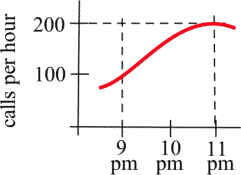
\includegraphics[width=0.3\textwidth]{img/chap5/image010.png}
    \caption{Calls per hour between 9 pm and 11 pm.}
    \label{fig:5-3-calls}
\end{figure}

\begin{solution}
We know that the accumulated calls will be the area under this rate graph over that two-hour period, the definite integral of this rate from $t=9$ to $t=11$.

The total number of calls will be $\displaystyle\int_9^{11}r(t)\,dt$.

The top of the area in Figure \ref{fig:5-3-callsapprox} is a curve, so we can’t get an exact answer. But we can approximate the area using rectangles. Let's choose to use four rectangles and left-endpoints.

\begin{figure}[!ht]
  \centering
    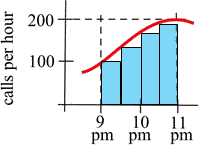
\includegraphics[width=0.4\textwidth]{img/chap5/image066.png}
    \caption{Approximating the number of calls between 9 pm and 11 pm.}
    \label{fig:5-3-callsapprox}
\end{figure}
$$\int_9^{11}r(t)\,dt\approx   0.5(100+150+180+195)=312.5 \enspace .$$
The units are (calls per hour)$\times$hours $=$ calls. Our estimate is that about 312 calls were made between 9 pm and 11 pm. Is this an under-estimate or an over-estimate?
\end{solution}\end{example}

\begin{example}
Describe the area between the graph of $f(x)=\dfrac{1}{x}$, the $x$-axis, and the vertical lines at $x=1$ and $x=5$ as a definite integral.

\begin{solution}
This is the same area we estimated to be about 1.68 before. Now we can use the notation of the definite integral to describe it. Our estimate of $\displaystyle\int_1^5\frac{1}{x}\,dx$ was 1.68. The true value of $\displaystyle\int_1^5\frac{1}{x}\,dx$ is about 1.61.
\end{solution}\end{example}

\begin{example}
Using the idea of area, determine the value of $\displaystyle\int_1^3(1+x)\,dx$.

\begin{solution}
  $\displaystyle\int_1^3(1+x)\,dx$ represents the area between the graph of $f(x)=1+x$, the $x$-axis, and the vertical lines at 1 and 3.

  \begin{figure}[!ht]
    \centering
      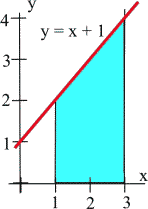
\includegraphics[width=0.3\textwidth]{img/chap5/image011.png}
      \caption{Calls per hour between 9 pm and 11 pm.}
      \label{fig:5-3-1plusx}
  \end{figure}
Since this area can be broken into a rectangle and a triangle, we can find the area exactly. The area equals
$4+\dfrac{1}{2}(2)(2)=6$.
\end{solution}\end{example}

\begin{example}
Table \ref{tab:5-3-population} shows rates of population growth for Berrytown for several years. Use this table to estimate the total population growth from 1970 to 2000:
\begin{table}[ht!]
  \centering
\begin{tabular}{lllll}
  \toprule
Year, $t$ &	1970 &	1980 &	1990 &	2000 \\
\midrule
Rate of population growth $R(t)$ in thousands of people per year &	1.5 &	1.9 &	2.2 &	2.4\\
\bottomrule
\end{tabular}
\caption{Population growth of Berrytown from 1970 to 2000.}
\label{tab:5-3-population}
\end{table}

\begin{solution}
The definite integral of this rate will give the total change in population over the thirty-year period. We only have a few pieces of information, so we can only estimate. Even though we haven't made a graph, we're still approximating the area under the rate curve, using rectangles. How wide are the rectangles? We have information every 10 years, so the rectangles have a width of 10 years. How many rectangles? Be careful here – this is a thirty-year span, so there are three rectangles.
  \begin{itemize}
    \item Using left-hand endpoints: $(1.5)(10) + (1.9)(10) + (2.2)(10) = 56$.
    \item Using right-hand endpoints: $(1.9)(10) + (2.2)(10) + (2.4)(10) = 65$.
  \end{itemize}
Taking the average of these two:
$$\dfrac{56+65}{2} = 60.5 \enspace .$$
Our best estimate of the total population growth from 1970 to 2000 is 60.5 thousand people.
\end{solution}\end{example}

\subsection{Signed Area}
You may have noticed that until this point, we've insisted that the integrand (the function we're integrating) be positive. That’s because we've been talking about area, which is always positive.

If the height (from the function) is a negative number, then multiplying it by the width doesn't give us actual area, it gives us the area with a negative sign.

But it turns out to be useful to think about the possibility of negative area. We’ll expand our idea of a definite integral now to include integrands that might not always be positive. The heights of the rectangles, the values from the function, now might not always be positive.

\begin{definition}[The Definite Integral and Signed Area]
The {\bf definite integral}\index{Definite integral}\index{Integral!definite} of a function $f(x)$ over an interval $[a,b]$ is the {\bf signed area}\index{Signed area}\index{Area!signed} between the curve $y=f(x)$, the $x$-axis, $x=a$ and $x=b$.

The {\bf definite integral} of a function $f(x)$ from $a$ to $b$ is the {\bf signed area} under the curve between $a$ and $b$.
\end{definition}
If the function is positive, the signed area is positive, as before (and we can call it area.)

If the function dips below the $x$-axis, the areas of the regions below the $x$-axis here will be negative. In this case, we cannot call it simply ``area.'' These negative areas take away from the definite integral.

$$\int_a^bf(x)\,dx = (\text{Area above } x\text{-axis}) - (\text{Area below }x\text{-axis})$$

If $f(t)$ represents a positive rate (in $y$-units per $t$-units), then the definite integral of $f(t)$ from $a$ to $b$ is the total $y$-units that accumulate between $t=a$ and $t=b$.

If $f(t)$ represents any rate (in $y$-units per $t$-units), then the definite integral of $f(t)$ from $a$ to $b$ is the net $y$-units that accumulate between $t=a$ and $t=b$.

\begin{example}
Find the definite integral of $f(x)=-2$ over the interval $[1,4]$.

\begin{figure}[!ht]
  \centering
    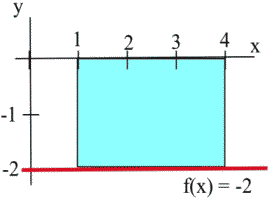
\includegraphics[width=0.3\textwidth]{img/chap5/image012.png}
    \caption{A region with negative signed area.}
    \label{fig:5-3-negative}
\end{figure}

\begin{solution}
$\displaystyle\int_1^4 -2\,dx$ is the signed area of the region shown in Figure \ref{fig:5-3-negative}. The region lies below the $x$-axis, so the area, 6, comes in with a negative sign. So the definite integral is $\displaystyle\int_1^4-2\,dx = -6$.
\end{solution}\end{example}

Negative rates indicate that the amount is decreasing. For example, if $f(t)$ is the velocity\index{Velocity} of a car in the positive direction along a straight line at time $t$ (miles/hour), then negative values of $f$ indicate that the car is traveling in the negative direction, backwards. The definite integral of $f$ is the net change in position of the car during the time interval. If the velocity is positive, positive distance accumulates. If the velocity is negative, distance in the negative direction accumulates.

This is true of any rate. For example, if $f(t)$ is the rate of population change (in people/year) for a town, then negative values of $f$ would indicate that the population of the town was getting smaller, and the definite integral (now a negative number) would be the change in the population, a decrease, during the time interval.

\begin{example}
In 1980 there were 12,000 ducks nesting around a lake, and the rate of population change (in ducks per year) is shown in Figure \ref{fig:5-3-ducks}. Write a definite integral to represent the total change in the duck population from 1980 to 1990, and estimate the population in 1990.

\begin{figure}[!ht]
  \centering
    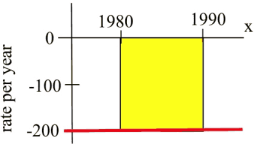
\includegraphics[width=0.3\textwidth]{img/chap5/image013.png}
    \caption{Rate of change in duck population from 1980 to 1990.}
    \label{fig:5-3-ducks}
\end{figure}

\begin{solution}
The change in population is:
\begin{align*}
  \int_{1980}^{1990}f(t)\,dt &= -(\text{area between }f\text{ and axis}) \\
    &\approx   -(200 \text{ducks/year})\cdot(10\text{ years})\\
    &= -2000\text{ ducks.}
  \end{align*}
Then (1990 duck population) $=$ (1980 population) $+$ (change from 1980 to 1990) $= (12000) + (-2000) = 10000$ ducks.
\end{solution}\end{example}

\begin{example}
A bug starts at the location $x=12$ on the $x$-axis at 1 pm walks along the axis with the velocity $v(x)$ shown in the graph in Figure \ref{fig:5-3-bug}. How far does the bug travel between 1 pm and 3 pm, and where is the bug at 3 pm?

\begin{figure}[!ht]
  \centering
    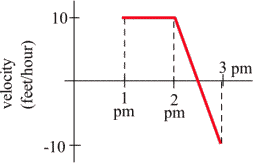
\includegraphics[width=0.3\textwidth]{img/chap5/image014.png}
    \caption{Velocity of a bug from 1 pm to 3 pm.}
    \label{fig:5-3-bug}
\end{figure}

\begin{solution}
Note that the velocity is positive from 1 until 2:30, then becomes negative. So the bug moves in the positive direction from 1 until 2:30, then turns around and moves back toward where it started. The area under the velocity curve from 1 to 2:30 shows the total distance traveled by the bug in the positive direction; the bug moved 12.5 feet in the positive direction. The area between the velocity curve and the $x$-axis, between 2:30 and 3, shows the total distance traveled by the bug in the negative direction, back toward home; the bug traveled 2.5 feet in the negative direction. The definite integral of the velocity curve, $\displaystyle\int_1^3v(t)\,dt$, shows the net change in distance:
$$\int_1^3v(t)\,dt = 12.5-2.5 = 10 \enspace .$$
The bug ended up 10 feet farther in the positive direction than he started. At 3 pm, the bug is at $x=22$.
\end{solution}\end{example}

\begin{example}
\label{ex:5-3-areas}
Use the graph in Figure \ref{fig:5-3-areas} to calculate $\displaystyle\int_0^2f(x)\,dx$, $\displaystyle\int_2^4f(x)\,dx$, $\displaystyle\int_4^5f(x)\,dx$, and $\displaystyle\int_0^5f(x)\,dx$.

\begin{figure}[!ht]
  \centering
    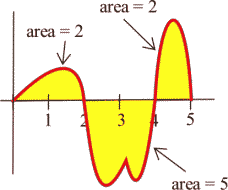
\includegraphics[width=0.3\textwidth]{img/chap5/image015.png}
    \caption{Graph for Example \ref{ex:5-3-areas}.}
    \label{fig:5-3-areas}
\end{figure}

\begin{solution}
Using the given areas, $\int_0^2f(x)\,dx = 2$, $\int_2^4f(x)\,dx = -5$, $\int_4^5f(x)\,dx = 2$, and $\int_0^5f(x)\,dx  = (\text{area above})-(\text{area below}) = (2+2)-(5)=-1$.
\end{solution}\end{example}

\section{The Fundamental Theorem of Calculus}
\label{sec:fund-theorem}
% From Section 3.2.
This section contains the most important and most used theorem of calculus, the Fundamental Theorem of Calculus. Discovered independently by Newton and Leibniz in the late 1600s, it establishes the connection between derivatives and integrals, provides a way of easily calculating many integrals, and was a key step in the development of modern mathematics to support the rise of science and technology. Calculus is one of the most significant intellectual structures in the history of human thought, and the Fundamental Theorem of Calculus is a most important brick in that beautiful structure.

\begin{theorem}[The Fundamental Theorem of Calculus]
Let $f(x)$ be a function whose derivative is continuous on an interval $[a, b]$. Then
$$\int_a^b f'(x)\,dx = f(b)-f(a) \enspace .$$
\end{theorem}
This is actually not new for us; we've been using this relationship for some time; we just haven't written it this way. This says what we've said before: the definite integral of a rate from $a$ to $b$ is the net $y$-units, the change in $y$, that accumulate between $x=a$ and $x=b$. Here we've just made it plain that that the rate is a derivative.

Thinking about the relationship this way gives us the key to finding exact answers for some definite integrals. If the integrand is the derivative of some function $f$, then maybe we could simply find $f$ and subtract. That would be easier than approximating with rectangles. Going backwards through the differentiation process will help us evaluate definite integrals.

\begin{example}
Find $f(x)$ if $f'(x)=2x$.

\begin{solution}
Oooh, I know this one. It's $f(x)=x^2+3$. Oh, wait, you were thinking something else? Yes, I guess you're right -- $f(x)=x^2$ works too. So does $f(x)=x^2-\pi$, and $f(x)=x^2+104589.2$. In fact, there are lots of answers.
\end{solution}\end{example}

In fact, there are infinitely many functions that all have the same derivative. And that makes sense – the derivative tells us about the shape of the function, but it doesn't tell about the location. We could shift the graph up or down and the shape wouldn't be affected, so the derivative would be the same.

This leads to one of the trickier definitions – pay careful attention to the articles (the versus an), because they're important.

\begin{definition}[Antiderivatives]
An {\bf antiderivative}\index{Antiderivative} of a function $f(x)$ is any function $F(x)$ where $F'(x)=f(x)$.

The antiderivative of a function $f(x)$ is a whole family of functions, written $F(x)+C$, where $F'(x)=f(x)$ and $C$ represents any constant (i.e., a real number).

The antiderivative of $f(x)$ is also called the {\bf indefinite integral}\index{Indefinite integral}\index{Integral!indefinite} of $f(x)$.

{\bf Notation for the Antiderivative}
The antiderivative of $f$ is written
$$\int f(x)\,dx$$
This notation resembles the definite integral, because the Fundamental Theorem of Calculus says antiderivatives and definite integrals are intimately related. But in this notation, there are no limits of integration.

The $\int$ symbol is still called an {\bf integral sign}; the $dx$  on the end still must be included; you can still think of $\int$ and $dx$  as left and right parentheses. The function $f$ is still called the {\bf integrand}.

{\bf Verb Forms}
We {\bf antidifferentiate}, or {\bf integrate}\index{Integrate}, or {\bf find the indefinite integral} of a function. This process is called {\bf antidifferentiation} or {\bf integration}\index{Integration}.
\end{definition}

There are no small families in the world of antiderivatives: if $f$ has one antiderivative $F$, then $f$ has an infinite number of antiderivatives and every one of them has the form $F(x)+C$.

\begin{example}
Find an antiderivative of $2x$.
\begin{solution}
We can choose any function we like as long as its derivative is $2x$, so we can pick, say, $F(x)=x^2-5.2$.
\end{solution}\end{example}

\begin{example}
Find the antiderivative of $2x$.

\begin{solution}
  Now we need to write the entire family of functions whose derivatives are $2x$. We can use the $\int$ notation:
$$\int 2x\,dx = x^2+C \enspace .$$
(Don't forget the $+C$!)
\end{solution}\end{example}

\begin{example}
Find $\int e^x\,dx$.

\begin{solution}
This is likely one you remember: $e^x$ is its own derivative, so it is also its own antiderivative. The integral sign tells us that we need to include the entire family of functions, so we need that $+C$ on the end:
$$\int e^x\,dx = e^x+C \enspace .$$
\end{solution}\end{example}

\subsection{Antiderivatives Graphically or Numerically}
Another way to think about the Fundamental Theorem of Calculus is to solve the expression for $F(b)$:

\begin{theorem}[The Fundamental Theorem of Calculus (restated)]
$$\int_a^b F'(x)\,dx = F(b)-F(a) \enspace .$$
The definite integral of a derivative from $a$ to $b$ gives the net change in the original function.

$$F(b)=F(a)+\int_a^b F'(x)\,dx$$
The amount we end up is the amount we start with plus the net change in the function.

This lets us get values for the antiderivative – as long as we have a starting point, and we know something about the area.

\begin{example}
Suppose $F(t)$ has the derivative $f(t)$ shown below, and suppose that we know $F(0)=5$. Find values for $F(1)$, $F(2)$, $F(3)$, and $F(4)$.

derivative graph
\begin{solution}
Using the second way to think about the Fundamental Theorem of Calculus, $F(b)=F(a)+\int_a^b F'(x)\,dx$, we can see that $F(1)=F(0)+\int_0^1 f(x)\,dx$. We know the value of $F(0)$, and we can easily find $\int_0^1 f(x)\,dx$ from the graph – it's just the area of a triangle. So
\begin{align*}
F(1) &= 5+0.5=5.5 \\
F(2) &= F(0)+\int_0^2 f(x)\,dx \\
    &= 5+1=6
\end{align*}
Note that we can start from any place of which we know the value; for example, now that we know $F(2)$, we can use that to find
\begin{align*}
F(3) &= F(2)+\int_2^3 f(x)\,dx \\
  &= 6-0.5 = 5.5 \\
F(4) &= F(3)+\int_3^4 f(x)\,dx  \\
  &= 5.5-1=4.5
\end{align*}
\end{solution}\end{example}

\begin{example}
The graph of $F'(t)=f(t)$ is shown in Figure [REF] below. Where does $F(t)$ have maximum and minimum values on the interval $[0, 4]$?

graph
\begin{solution}
Since $F(b)=F(a)+\int_a^b F'(x)\,dx$, we know that $F$ is increasing as long as the area accumulating under $y = F'(t)=f(t)$ is positive (until $t=3$), and then decreases when the curve dips below the $t$-axis so that negative area starts accumulating. The area between $t=3$ and $t=4$ is much smaller than the positive area that accumulates between 0 and 3, so we know that $F(4)$ must be larger than $F(0)$. The maximum value is when $t=3$; the minimum value is when $t=0$.
\end{solution}\end{example}

Note that this is a different way to look at a problem we already knew how to solve – in Chapter 2, we would have found critical points of $F$, where $f=0$: there's only one, when $t=3$. $f(t)=F'(t)$ goes from positive to negative there, so $F$ has a local max at that point. It's the only critical point, so it must be a global maximum. Then we would look at the values of $F$ at the endpoints to find which was the global minimum.

We can also attempt to sketch a function based on the graph of the derivative.

\begin{example}
The graph below shows $f'(x)$ – the rate of change of $f(x)$. Use it to sketch a graph of $f(x)$ that satisfies $f(0)=0$.

graph
\begin{solution}
Recall from Section \ref{sec:sketching} the relationships between the function graph and the derivative graph:
\begin{table}[ht!]
    \centering
    \begin{tabular}{*{5}{l}}
    \toprule
    $f(x)$ &	Increasing &	Decreasing &	Concave Up &	Concave Down	\\
    \midrule
    $f'(x)$	& $+$ & $-$ &	Increasing & Decreasing \\
    \bottomrule
    \end{tabular}
    \caption{The relationship between a function and its derivative.}
    \label{tab:5-derivs}
\end{table}

In the graph shown, we can see the derivative is positive on the interval $(0, 1)$ and $(3,\infty)$, so the graph of $f$ should be increasing on those intervals. Likewise, $f$ should be decreasing on the interval $(1,3)$.

In the graph, $f'$ is decreasing on the interval $(0, 2)$, so $f$ should be concave down on that interval. Likewise, $f$ should be concave up on the interval $(2,\infty)$.

The derivative itself is not enough information to know where the function $f$ starts, since there are a family of antiderivatives, but in this case we are given a specific point at which to start.

To start the sketch, we might note first the shapes we need:

graph
then sketch the basic shapes:

graph
Now we can attempt to sketch the graph, starting at the point $(0, 0)$. Notice we are very roughly sketching this, as we don't have much information to work with. We can tell, though, from the graph that the area from $x=0$ to $x=1$ is about the same as the area from $x=1$ to $x=3$, so we would expect the net area from $x=0$ to $x=3$ to be close to 0.

graph
It turns out this graph isn't horribly bad. Smoothing it out would give a graph closer to the actual antiderivative graph, shown below.

graph
\end{solution}\end{example}

\subsection{Derivative of the Integral}
There is another important connection between the integral and derivative.

\begin{theorem}[The Fundamental Theorem of Calculus (Part 2)]
If
$$A(x)=\int_a^x f(t)\,dt$$
then
$$A'(x)=\frac{d}{dx} \int_a^x f(t)\,dt = f(x) \enspace .$$
I.e., the derivative of the accumulation function is the original function.

\begin{example}
Let $F(x)=\int_0^x f(t)\,dt$, where $f$ is graphed below. Estimate $F'(3)$.

graph
\begin{solution}
The function $F(x)$ measures the area from $t=0$ to some $t=x$. To estimate $F'(3)$, we want to estimate how much the area is increasing when $t=3$. Since the value of the function $f(t)$ is 0 at $t=3$, the area will not be increasing or decreasing, so we can estimate $F'(3)=0$.

Directly using the fundamental theorem of calculus part 2,
$$F'(x) = \frac{d}{dx} \int_a^xf(t)\,dt = f(x) $$
so
$$F'(x)=f(3)=0 \enspace .$$
\end{solution}\end{example}

\section{Integral Formulas}
\label{sec:formulas}
% From Section 3.3
Now we can put the ideas of areas and antiderivatives together to get a way of evaluating definite integrals that is exact and often easy. To evaluate a definite integral ∫abf(t)dt, we can find any antiderivative F(t) of f(t) and evaluate F(b)-F(a). The problem of finding the exact value of a definite integral reduces to finding some (any) antiderivative F of the integrand and then evaluating F(b)-F(a). Even finding one antiderivative can be difficult, and we will stick to functions that have easy antiderivatives.

Building Blocks
Antidifferentiation is going backwards through the derivative process. So the easiest antiderivative rules are simply backwards versions of the easiest derivative rules. Recall from Chapter 2:

Derivative Rules: Building Blocks
In what follows, f and g are differentiable functions of x.

Constant Multiple Rule
ddx(kf)=kf′
Sum and Difference Rule
ddx(f±g)=f′±g′
Power Rule
ddx(xn)=nxn-1
Special cases:
ddx(k)=0(Because k=kx0.)
ddx(x)=1(Because x=x1.)
Exponential Functions
ddx(ex)=ex
ddx(ax)=ln(a)ax
Natural Logarithm
ddx(ln(x))=1x
Thinking about these basic rules was how we came up with the antiderivatives of 2x and ex before.

The corresponding rules for antiderivatives are next – each of the antiderivative rules is simply rewriting the derivative rule. All of these antiderivatives can be verified by differentiating.

There is one surprise – the antiderivative of 1x is actually not simply ln(x), it's ln|x|. This is a good thing – the antiderivative has a domain that matches the domain of 1x, which is bigger than the domain of ln(x), so we don’t have to worry about whether our x's are positive or negative. But we must be careful to include those absolute values – otherwise, we could end up with domain problems.

Antiderivative Rules: Building Blocks
In what follows, f and g are differentiable functions of x, and k, n, and C are constants.

Constant Multiple Rule
∫k⋅f(x)dx=k⋅∫f(x)dx
Sum and Difference Rule
∫(f(x)±g(x))dx=∫f(x)dx±∫g(x)dx
Power Rule
∫xndx=xn+1n+1, provided that n≠-1
Special case:
∫kdx=kx+C(Because k=kx0.)
(The other special case (n=-1) is covered next.)

Natural Logarithm
∫x-1dx=∫1xdx=ln|x|+C
Exponential Functions
∫exdx=ex+C
∫axdx=axln(a)+C
\begin{example}
Find the antiderivative of y=3x7-15x--√+14x2.

\begin{solution}
∫(3x7-15x--√+14x2)dx===∫(3x7-15x1/2+14x-2)dx3x88-15x3/23/2+14x-1-1+C38x8-10x3/2-14x-1+C
\end{solution}\end{example}

\begin{example}
Find ∫(ex+12-16x)dx.

\begin{solution}
  ∫(ex+12-16x)dx=ex+12x-16ln|x|+C
\end{solution}\end{example}

\begin{example}
Find F(x) so that F′(x)=ex and F(0)=10.

\begin{solution}
This time we are looking for a particular antiderivative; we need to find exactly the right constant. Let's start by finding the antiderivative:
∫exdx=ex+C
So we know that F(x)=ex+(some constant), now we just need to find which one. To do that, we'll use the other piece of information (the initial condition):
F(x)=F(0)=C=ex+Ce0+C=1+C=109
The particular constant we need is 9; thus, F(x)=ex+9.
\end{solution}\end{example}

The reason we are looking at antiderivatives right now is so we can evaluate definite integrals exactly. Recall the Fundamental Theorem of Calculus:

∫abF′(x)dx=F(b)-F(a)
If we can find an antiderivative for the integrand, we can use that to evaluate the definite integral. The evaluation F(b)-F(a) is represented as F(x)]ba or F(x)|ba.

\begin{example}
Evaluate ∫13xdx in two ways:

\begin{solution}
By sketching the graph of y=x and geometrically finding the area.
By finding an antiderivative of F(x) of the integrand and evaluating F(3)-F(1).
The graph of y=x is shown below, and the shaded region corresponding to the integral has area 4.

graph
One antiderivative of x is F(x)=12x2, and
∫13xdx====[12x2]31(12(3)2)-(12(1)2)92-124.
Note that this answer agrees with the answer we got geometrically.

If we had used another antiderivative of x, say F(x)=12x2+7, then
∫13xdx====[12x2+7]31(12(3)2+7)-(12(1)2+7)92+7-12-74.
In general, whatever constant we choose gets subtracted away during the evaluation, so we might as well always choose the easiest one, where the constant is 0.
\end{solution}\end{example}

\begin{example}
Find the area between the graph of y=3x2 and the horizontal axis for x between 1 and 2.

\begin{solution}
  This is
∫123x2dx=x3∣∣21=23-13=7.
\end{solution}\end{example}

\begin{example}
A robot has been programmed so that when it starts to move, its velocity after t seconds will be 3t2 feet/second.

\begin{solution}
How far will the robot travel during its first 4 seconds of movement?
How far will the robot travel during its next 4 seconds of movement?
The distance during the first 4 seconds will be the area under the graph of velocity, from t=0 to t=4.

graph
That area is the definite integral ∫043t2dt. An antiderivative of 3t2 is t3, so ∫043t2dt=t3]40=43-03=64 feet.

∫483t2dt=t3]84=83-43=512-64=448 feet.
\end{solution}\end{example}

\begin{example}
Suppose that t minutes after putting 1000 bacteria on a Petri plate the rate of growth of the population is 6t bacteria per minute.

\begin{solution}
How many new bacteria are added to the population during the first 7 minutes?
What is the total population after 7 minutes?
The number of new bacteria is the area under the rate of growth graph, and one antiderivative of 6t is 3t2.

graph
So
new bacteria=∫076tdt=3t2∣∣70=3(7)2-3(0)2=147
The new population = (old population) + (new bacteria) = 1000 + 147 = 1147 bacteria.
\end{solution}\end{example}

\begin{example}
A company determines their marginal cost for production, in dollars per item, is MC(x)=4x√+2 when producing x thousand items. Find the cost of increasing production from 4 thousand items to 5 thousand items.

\begin{solution}
  Remember that marginal cost is the rate of change of cost, and so the fundamental theorem tells us that ∫abMC(x)dx=∫abC′(x)dx=C(b)-C(a). In other words, the integral of marginal cost will give us a net change in cost. To find the cost of increasing production from 4 thousand items to 5 thousand items, we need to integrate ∫45MC(x)dx.

We can write the marginal cost as MC(x)=4x-1/2+2. We can then use the basic rules to find an antiderivative:
C(x)=4x1/21/2+2x=8x--√+2x.
Using this,
Net change in cost ===\approx   ∫45(4x-1/2+2)dx[8x--√+2x]54(85–√+2(5))-(84–√+2(4))3.889
It will cost 3.889 thousand dollars to increase production from 4 thousand items to 5 thousand items. (The final answer would be better written as \$3889.)
\end{solution}\end{example}

\section{Integration by Substitution}
\label{sec:substitution}
% From Section 3.4
We don't have many integration rules. For quite a few of the problems we see, the rules won't directly apply; we'll have to do some algebraic manipulation first. In practice, it is much harder to write down the antiderivative of a function than it is to find a derivative. (In fact, it's very easy to write a function that doesn't have any antiderivative you can find with algebra, although proving that it doesn't have an antiderivative is much more difficult.)

The Substitution Method (also called u-Substitution) is one way of algebraically manipulating an integrand so that the rules apply. This is a way to unwind or undo the Chain Rule for derivatives. When you find the derivative of a function using the Chain Rule, you end up with a product of something like the original function times a derivative. We can reverse this to write an integral:
ddxf(g(x))=f′(g(x))g′(x)
so
f(g(x))=∫f′(g(x))g′(x)dx
With substitution, we will substitute u=g(x) (hence the name u-substitution). This means dudx=g′(x), so du=g′(x)dx. Making these substitutions, ∫f′(g(x))g′(x)dx becomes ∫f′(u)du, which will probably be easier to integrate.

Try u-Substitution when you see a product in your integral, especially if you recognize one factor as the derivative of some part of the other factor.

The u-Substitution Method for Antiderivatives
The goal is to turn ∫f(g(x))dx into ∫f(u)du, where f(u) is much less messy than f(g(x)).

Let u be some part of the integrand. A good first choice is one step inside the messiest bit.
Compute du=dudxdx.
Translate all your x's into u's everywhere in the integral, including the dx. When you're done, you should have a new integral that is entirely in u. If you have any x's left, then that's an indication that the substitution didn't work or isn't complete; you may need to go back to step 1 and try a different choice for u.
Integrate the new u-integral, if possible. If you still can't integrate it, go back to step 1 and try a different choice for u.
Finally, substitute back x's for u's everywhere in your answer.
\begin{example}
Evaluate ∫x4-x2√dx.

\begin{solution}
  This integrand is more complicated than anything in our list of basic integral formulas, so we'll have to try something else. The only tool we have is substitution, so let's try that!

Let u be some part of the integrand. A good first choice is one step inside the messiest bit:

Let u=4-x2.

Compute du=dudxdx:

du=-2xdx. There is xdx in the integrand, so that’s a good sign; that will be -12du.

Translate all your x's into u's everywhere in the integral, including the dx:

∫x4-x2-----√dx====∫14-x2-----√(xdx)∫1u--√(-12du)-12∫1u--√du-12∫u-1/2du
Alternatively, we could have solved for dx and substituted that and simplified: dx=du-2x, so
∫x4-x2-----√dx====∫xu--√(du-2x)∫1u--√(-12du)-12∫1u--√du-12∫u-1/2du
Integrate the new u-integral, if possible:

-12∫u-1/2du=-12u1/21/2+C=-u1/2+C
Finally, substitute back x's for u's everywhere in the answer:

Undoing our u=4-x2 substitution yields
-u1/2+C=-4-x2-----√+C.
Thus we have found
∫x4-x2-----√dx=-4-x2-----√+C
How would we check this? By differentiating:
ddx(-4-x2-----√+C)====ddx(-(4-x2)1/2+C)-12(4-x2)-1/2(-2x)x(4-x2)-1/2x4-x2-----√
\end{solution}\end{example}

\begin{example}
Evaluate ∫exdx(ex+15)3

\begin{solution}
This integral is not in our list of building blocks. But notice that the derivative of ex+15 (which we see in the denominator) is just ex (which we see in the numerator), so substitution will be a good choice for this.

Let u=ex+15. Then du=exdx, and this integral becomes ∫duu3=∫u-3du.

Luckily, that is on our list of building block formulas: ∫duu3=u-2-2+C=-12u2+C.

Finally, translating back:
∫exdx(ex+15)3=-12(ex+15)2+C.
\end{solution}\end{example}

\begin{example}
Evaluate

∫x2x3+5dx
∫x3+5x2dx

\begin{solution}
  This is not a basic integral, but the composition is less obvious. Here, we can treat the denominator as the inside of the 1x function.

Let u=x3+5. Then du=3x2dx. Solving for dx, dx=du3x2. Substituting,
∫x2x3+5dx=∫x2udu3x2=∫1udu3=13∫1udu
Using our basic formulas,
13∫1udu=13ln|u|+C.
Undoing the substitution,
∫x2x3+5dx=13ln∣∣x3+5∣∣+C.
It is tempting to start this problem the same way we did the last, but if we try it will not work, since the numerator of this fraction is not the derivative of the denominator. Instead, we need to try a different approach. For this problem, we can use some basic algebra:
∫x3+5x2dx==∫(x3x2+5x2)dx∫(x+5x-2)dx.
We can integrate this using our basic rules, without needing substitution:
∫(x+5x-2)dx==x22+5x-1-1+C12x2-5x+C.
\end{solution}\end{example}

Substitution and Definite Integrals
When you use substitution to help evaluate a definite integral, you have a choice for how to handle the limits of integration. You can do either of these, whichever seems better to you. The important thing to remember is that the original limits of integration were values of the original variable (say, x), not values of the new variable (say, u).

You can solve the antiderivative as a side problem, translating back to x’s, and then use the antiderivative with the original limits of integration.

Or…

You can substitute for the limits of integration at the same time as you’re substituting for everything inside the integral, and then skip the translate back into x step.

If the original integral had endpoints x=a and x=b, and we make the substitution u=g(x) and du=g′(x)dx, then the new integral will have endpoints u=g(a) and u=g(b) and
∫x=bx=a(original integrand)dx
becomes
∫u=g(b)u=g(a)(new integrand)du.
Method 1 seems more straightforward for most students, but it can involve some messy algebra. Method 2 is often neater and usually involves fewer steps.

\begin{example}
Evaluate ∫01(3x-1)4dx.

\begin{solution}
We'll need substitution to find an antiderivative, so we'll need to handle the limits of integration carefully. Let's solve this example both ways.

Doing the antiderivative as a side problem:

Step One – find the antiderivative, using substitution:

Let u=3x-1. Then du=3dx and
∫(3x-1)4dx=∫u4(13du)=13u55+C.
Translating back to x:
13u55+C=(3x-1)515+C.
Step Two – evaluate the definite integral:
∫01(3x-1)4dx=(3x-1)515]10=(3(1)-1)515-(3(0)-1)515=3215--115=3315.
Substituting for the limits of integration:

Let u=3x-1. Then du=3dx and, substituting for the limits of integration, when x=0, u=-1, and when x=1, u=2.

So,
∫x=1x=0(3x-1)4dx=====∫u=2u=-1u4(13du)u515]u=2u=-1(2)515-(-1)5153215--1153315
\end{solution}\end{example}

\begin{example} 
Evaluate ∫210(ln(x))6xdx.

\begin{solution}
  I can see the derivative of ln(x) in the integrand, so I can tell that substitution is a good choice.

Let u=ln(x). Then du=1xdx. When x=2, u=ln(2). When x=10, u=ln(10). So the new definite integral is
∫x=2x=10(ln(x))6xdx===\approx   ∫u=ln(2)u=ln(10)u6duu77]u=ln(10)u=ln(2)17((ln(10))7-(ln(2))7)49.01.
\end{solution}\end{example}

\section{Integration by Parts}
\label{sec:integration-by-parts}
% Section 3.5
%\subsection{Integration By Parts}
{\bf Integration by parts}\index{Integration by parts} is an integration method which enables us to find antiderivatives of some new functions such as $\ln(x)$ as well as antiderivatives of products of functions such as $x^2\ln(x)$ and $xe^x$.

If the function we're trying to integrate can be written as a product of two functions, $u$, and $dv$, then integration by parts lets us trade out a complicated integral for hopefully simpler one.

\begin{theorem}[Integration by Parts Formula]
$$\int u\,dv=uv-\int v\,du$$
For definite integrals:
$$\int_a^bu\,dv = \left.uv\right|_a^b - \int_a^b v \,du$$
\end{theorem}
\begin{example}
Integrate $\displaystyle\int xe^x\,dx$.

\begin{solution}
To use the Integration by Parts method, we break apart the product into two parts:
$$u=x\quad \text{and}\quad dv=e^x\,dx \enspace .$$
We now calculate $du$, the derivative of $u$, and $v$, the integral of $dv$:
$$du = \left(\frac{d}{dx}x\right)\,dx \quad \text{and} \quad v = \int e^x\,dx = e^x \enspace .$$
Using the Integration by Parts formula,
$$\int xe^x\,dx = uv-\int v\,du = xe^x - \int e^x\,dx \enspace . $$
Notice the remaining integral is simpler that the original, and one which we can easily evaluate:
$$xe^x-\int e^x\,dx = xe^x - e^x + C \enspace .$$
\end{solution}\end{example}

In the last example we could have chosen either $x$ or $e^x$ as our $u$, but had we chosen $u=e^x$, the second integral would have become messier, rather than simpler.

\begin{note}[Rule of Thumb: LIATE]
When selecting the $u$ for Integration by Parts, a common rule of thumb is the ``LIATE" mnemonic. Choose $u$ in the following order of preference.
\begin{itemize}
  \item[L:] {\bf L}ogarithmic functions
  \item[I:] {\bf I}nverse trigonometric Functions
  \item[A:] {\bf A}lgebraic functions (polynomials, roots, etc.)
  \item[T:] {\bf T}rigonometic Functions
  \item[E:] {\bf E}xponential functions
\end{itemize}

\end{note}
\begin{example}
Integrate $\displaystyle\int_1^4 6x^2\ln(x)\,dx$.

\begin{solution}
Since this contains a logarithmic expression, we'll use it for our $u$.
$$u = \ln(x) \quad {\text and} \quad dv = 6x^2\,dx$$
We now calculate $du$ and $v$.
$$du = \frac{1}{x}\,dx  \quad {\text and} \quad v = \int 6x^2\,dx = 6\frac{x^3}{3} = 2x^3$$
Using the Integration By Parts formula, we have
$$\int_1^4 6x^2\ln(x)\,dx = \left.2x^3\ln(x)\right|^4_1-\int^4_1 6x^2 \frac{1}{x}\,dx \enspace .$$
We can simplify the expression in the integral on the right.
$$\int^4_1 6x^2\ln(x)\,dx = \left.2x^3\ln(x)\right|^4_1 - \int^4_1 6x\,dx$$
The remaining integral is a basic one we can now evaluate.
$$\int^4_1 6x^2\ln(x)\,dx = \left.2x^3\ln(x)\right|^4_1 - \left.3x^2\right|^4_1$$
Finally, we can evaluate the expressions.
\begin{align*}
\int^4_1 6x^2\ln(x)\,dx &= ((2\cdot 4^3\ln(4))-(2\cdot 1^3\ln(1)))-((3\cdot 4^2)-(3\cdot 1^2)) \\
&= 128\ln(4)-45\\
&\approx   132.446
\end{align*}
\end{solution}\end{example}

\section{Applications of Integrals}
\label{sec:integral-applications}

% From Sections 3.7 and 3.6

Consumer and Producer Surplus
Here are a demand and a supply curve for a product. Which is which?

graph
The demand curve is decreasing – lower prices are associated with higher quantities demanded, higher prices are associated with lower quantities demanded. Demand curves are often shown as if they were linear, but there’s no reason they have to be.

The supply curve is increasing – lower prices are associated with lower supply, and higher prices are associated with higher quantities supplied.

The point where the demand and supply curve cross is called the equilibrium point (q∗,p∗).

graph
Suppose that the price is set at the equilibrium price, so that the quantity demanded equals the quantity supplied. Now think about the folks who are represented on the left of the equilibrium point. The consumers on the left would have been willing to pay a higher price than they ended up having to pay, so the equilibrium price saved them money. On the other hand, the producers represented on the left would have been willing to supply these goods for a lower price – they made more money than they expected to. Both of these groups ended up with extra cash in their pockets!

Graphically, the amount of extra money that ended up in consumers' pockets is the area between the demand curve and the horizontal line at p∗. This is the difference in price, summed up over all the consumers who spent less than they expected to – a definite integral. Notice that since the area under the horizontal line is a rectangle, we can simplify the area integral:
∫0q∗(d(q)-p∗)dq=∫0q∗d(q)dq-∫0q∗p∗dq=∫0q∗d(q)dq-p∗q∗.
The amount of extra money that ended up in producers' pockets is the area between the supply curve and the horizontal line at p∗. This is the difference in price, summed up over all the producers who received more than they expected to. Similar to consumer surplus, this integral can be simplified:
∫0q∗(p∗-s(q))dq=∫0q∗p∗dq-∫0q∗s(q)dq=p∗q∗-∫0q∗s(q)dq.
Consumer and Producer Surplus
Given a demand function p=d(q) and a supply function p=s(q), and the equilibrium point (q∗,p∗)
The consumer surplus is
∫0q∗d(q)dq-p∗q∗.
The producer surplus is
p∗q∗-∫0q∗s(q)dq.
The sum of the consumer surplus and producer surplus is the total gains from trade.
What are the units of consumer and producer surplus? The units are (price per item)(quantity of items) = money!

\begin{example}
Suppose the demand for a product is given by p=d(q)=-0.8q+150 and the supply for the same product is given by p=s(q)=5.2q. For both functions, q is the quantity and p is the price, in dollars.

\begin{solution}
  Find the equilibrium point.
Find the consumer surplus at the equilibrium price.
Find the producer surplus at the equilibrium price.
The equilibrium point is where the supply and demand functions are equal. Solving -0.8q+150=5.2q gives q=25.
The consumer surplus is
∫025(-0.8q+150)dq-(130)(25)=\$250.
The producer surplus is
(130)(25)-∫0255.2qdq=\$1625.
\end{solution}\end{example}

\begin{example}
The tables below show information about the demand and supply functions for a product. For both functions, q is the quantity and p is the price, in dollars.

q	0	100	200	300	400	500	600	700	p	70	61	53	46	40	35	31	28
q	0	100	200	300	400	500	600	700	p	14	21	28	33	40	47	54	61
Which is which? That is, which table represents demand and which represents supply?
What is the equilibrium price and quantity?
Find the consumer and producer surplus at the equilibrium price.

\begin{solution}
The first table shows decreasing price associated with increasing quantity, so that is the demand function. The second table shows increasing price associated with increasing quantity, so that is the supply function.
For both functions, q=400 is associated with p=40; the equilibrium price is \$40 and the equilibrium quantity is 400 units. Notice that we were lucky here, because the equilibrium point is actually one of the points shown. In many cases with a table, we would have to estimate.
The consumer surplus uses the demand function, which comes from the first table. We'll have to approximate the value of the integral using rectangles. There are 4 rectangles, and let's choose to use left endpoints.

The consumer surplus is
∫0400(demand)dq-(40)(400)\approx   (100)(70+61+53+46)-(40)(400)=\$7000
So the consumer surplus is about \$7000.

The producer surplus uses the supply function, which comes from the second table. Let's choose to use left endpoints for this integral also.

The producer surplus is
(40)(400)-∫0400(supply)dq\approx   (40)(400)-(100)(14+21+28+33)=\$6400
So the producer surplus is about \$6400.
\end{solution}\end{example}

Continuous Income Stream
In precalculus, you learned about compound interest in that really simple situation where you made a single deposit into an interest-bearing account and let it sit undisturbed, earning interest, for some period of time. Recall:

Compound Interest Formulas
Let P be the principal (initial investment), r be the annual interest rate expressed as a decimal, and A(t) be the amount in the account at the end of t years.

Compounding n times per year
A(t)=P(1+rn)nt
Compounded continuously
A(t)=Pert
If you’re using this formula to find what an account will be worth in the future, t>0 and A(t) is called the future value.

If you're using the formula to find what you need to deposit today to have a certain value P sometime in the future, t<0 and A(t) is called the present value.

You may also have learned somewhat more complicated annuity formulas to deal with slightly more complicated situations – where you make equal deposits equally spaced in time.

But real life is not usually so neat.

Calculus allows us to handle situations where deposits are flowing continuously into an account that earns interest. As long as we can model the flow of income with a function, we can use a definite integral to calculate the present and future value of a continuous income stream. The idea here is that each little bit of income in the future needs to be multiplied by the exponential function to bring it back to the present, and then we'll add them all up (a definite integral).

Continuous Income Stream
Suppose money can earn interest at an annual interest rate of r, compounded continuously. Let F(t) be a continuous income function (in dollars per year) that applies between year 0 and year T.

Then the present value of that income stream is given by
PV=∫0TF(t)e-rtdt.
The future value can be computed by the ordinary compound interest formula
FV=PVert.
This is a useful way to compare two investments – find the present value of each to see which is worth more today.

\begin{example}
You have an opportunity to buy a business that will earn \$75,000 per year continuously over the next eight years. Money can earn 2.8\% per year, compounded continuously. Is this business worth its purchase price of \$630,000?

\begin{solution}
  First, please note that we still have to make some simplifying assumptions. We have to assume that the interest rates are going to remain constant for that entire eight years. We also have to assume that the \$75,000 per year is coming in continuously, like a faucet dripping dollars into the business. Neither of these assumptions might be accurate.

But moving on: The present value of the \$630,000 is, well, \$630,000. This is one investment, where we put our \$630,000 in the bank and let it sit there.

To find the present value of the business, we think of it as an income stream. The function F(t) in this case is a constant \$75,000 dollars per year, so F(t)=75,000. The interest rate is 2.8\% and the term we're interested in is 8 years, so r=.028, and T=8:
PV=∫0875000e-0.028tdt\approx   537,548.75
The present value of the business is about \$537,500, which is less than the \$630,000 asking price, so this is not a good deal.
\end{solution}\end{example}

While this integral could have been done using substitution, for many of the integrals in this section we don't have the techniques to use antiderivatives or, in some cases, no antiderivative exists. Technology will work quickly, and it will give you an answer that is good enough.

\begin{example}
A company is considering purchasing a new machine for its production floor. The machine costs \$65,000. The company estimates that the additional income from the machine will be a constant \$7000 for the first year, then will increase by \$800 each year after that. In order to buy the machine, the company needs to be convinced that it will pay for itself by the end of 8 years with this additional income. Money can earn 1.7\% per year, compounded continuously. Should the company buy the machine?

\begin{solution}
  We'll assume that the income will come in continuously over the 8 years. We’ll also assume that interest rates will remain constant over that 8-year time period.

We're interested in the present value of the machine, which we will compare to its \$65,000 price tag. Let t be the time, in years, since the purchase of the machine. The income from the machine is different depending on the time.

From t=0 to t=1 (the first year), the income is constant \$7000 per year. From t=1 to t=8, the income is increasing by \$800 each year; the income flow function F(t) will be F(t)=7000+800(t-1)=6200+800t. To find the present value, we'll have to divide the integral into the two pieces, one for each of the functions:
PV=∫017000e-0.017tdt+∫18(6200+800t)e-0.017tdt\approx   70166.
The present value is greater than the cost of the machine, so the company should buy the machine.
\end{solution}\end{example}

\subsection{Average Value}
We know the average of n numbers a1,a2,…,an is their sum divided by n. But what if we need to find the average temperature over a day's time – there are too many possible temperatures to add them up! This is a job for the definite integral.

% From Section 3.6.
Average Value
The average value of a function f(x) on the interval [a,b] is given by
1b-a∫baf(x)dx.
The average value of a positive f has a nice geometric interpretation. Imagine that the area under f (graph (a) below) is a liquid that can leak through the graph to form a rectangle with the same area (graph (b) below).

If the height of the rectangle is H, then the area of the rectangle is H⋅(b-a). We know the area of the rectangle is the same as the area under f so H⋅(b-a)=∫baf(x)dx. Then
H=1b-a∫baf(x)dx,
the average value of f on [a,b].

The average value of a positive function f is the height H of the rectangle whose area is the same as the area under f.

\begin{example}
During a 9 hour work day, the production rate at time t hours after the start of the shift was given by the function r(t)=5+t√ cars per hour. Find the average hourly production rate.

\begin{solution}
The average hourly production is 19-0∫90(5+t√)dt=7 cars per hour.
\end{solution}\end{example}

A note about the units – remember that the definite integral has units (cars per hour)⋅(hours) = cars. But the 1b-a in front has units 1hours – the units of the average value are cars per hour, just what we expect an average rate to be.

In general…
…the average value of a function will have the same units as the integrand.

Function averages, involving means and more complicated averages, are used to smooth data so that underlying patterns are more obvious and to remove high frequency noise from signals. In these situations, the original function f is replaced by some average of f. If f is rather jagged time data, then the ten year average of f is the integral g(x)=110∫x-5x+5f(t)dt, an average of f over 5 units on each side of x.

For example, the figure below shows the graphs of a Monthly Average (rather “noisy” data) of surface temperature data, an Annual Average (still rather jagged), and a Five Year Average (a much smoother function).

graph by Robert A. Rohde
Image prepared by Robert A. Rohde, http://commons.wikimedia.org/wiki/File:Short_Instrumental_Temperature_Record.png.
Typically the average function reveals the pattern much more clearly than the original data. This use of a moving average value of noisy data (weather information, stock prices) is a very common.

\begin{example}  2
The graph below shows the amount of water in a reservoir over a 12 hour period. Estimate the average amount of water in the reservoir over this period.

graph
\begin{solution}
If V(t) is the volume of the water (in millions of liters) after t hours, then the average amount is 112∫120V(t)dt. In order to find the definite integral, we'll have to estimate. Let's use 6 rectangles and take the heights from their right edges (there's nothing special about using 6 rectangles or right edges – other choices would still give you a valid estimate).

graph
The estimate of the integral is
∫120V(t)dt\approx   (18)(2)+(9.7)(2)+(8.2)(2)+(12)(2)+(19.9)(2)+(22)(2)=179.6.
The units of this integral are (millions of liters)⋅(feet). So our estimate of the average volume is 112⋅179.6\approx   15 millions of liters. (The estimate might change a little depending on how we estimate the function values from the graph.)

In the figure below, you can see the same graph with the line y=15 drawn in. The area under the curve and the area under the rectangle are (approximately) the same.

graph
In fact, that would be a different way to estimate the average value. We could have estimated the placement of the horizontal line so that the area under the curve and under the line were equal.
\end{solution}\end{example}

Area
We have already used integrals to find the area between the graph of a function and the horizontal axis. Integrals can also be used to find the area between two graphs.

If f(x)≥g(x) for all x in [a,b], then we can approximate the area between f and g by partitioning the interval [a,b] and forming a Riemann sum, as shown in the picture. The height of each rectangle is top - bottom, f(ci)-g(ci) so the area of the i-th rectangle is (height)⋅(base) = (f(ci)-g(ci))⋅Δx. Adding up these rectangles gives an approximation of the total area as ∑ni=1(f(ci)-g(ci))⋅Δx, a Riemann sum.

grapg
The limit of this Riemann sum, as the number of rectangles gets larger and their width gets smaller, is the definite integral ∫ba(f(x)-g(x))dx.

Area Between Two Curves
The area between two curves f(x) and g(x), where f(x)≥g(x), between x=a and x=b is
∫ba(f(x)-g(x))dx.
The integrand is top - bottom. Make a graph or use test values to be sure which curve is which.

\begin{example}  3
Find the area bounded between the graphs of f(x)=x and g(x)=3 for 1≤x≤4.

graph
\begin{solution}
Always start with a graph so you can see which graph is the top and which is the bottom. In this example, the two curves cross, and they change positions; we’ll need to split the area into two pieces. Geometrically, we can see that the area is 2 + 0.5 = 2.5.

Writing the area as a sum of definite integrals, we get
Area =∫31(3-x)dx+∫43(x-3)dx.
These integrals are easy to evaluate using antiderivatives:
∫31(3-x)dx===[3x-x22]31(9-92)-(3-12)2
∫43(x-3)dx===[x22-3x]43(162-12)-(92-9)12
The sum of these two integrals tells us that the total area between f and g is 2.5 square units, which we already knew from the picture.
\end{solution}\end{example}

Note that the single integral ∫41(3-x)dx=1.5 is not the area we want in the last example. The value of the integral is 1.5, and the value of the area is 2.5. That's because for the triangle on the right, the graph of y=x is above the graph of y=3, so the integrand 3-x is negative; in the definite integral, the area of that triangle comes in with a negative sign.

In this example, it was easy to see exactly where the two curves crossed so we could break the region into the two pieces to figure separately. In other examples, you might need to solve an equation to find where the curves cross.

\begin{example}
Two objects start from the same location and travel along the same path with velocities vA(t)=t+3 and vB(t)=t2-4t+3 meters per second. How far ahead is A after 3 seconds?

graph
\begin{solution}
Since vA(t)≥vB(t) , the area between the graphs of vA and vB represents the distance between the objects.

After 3 seconds, the distance apart is
∫30(vA(t)-vB(t))dt=====∫30((t+3)-(t2-4t+3))dt∫30(5t-t2)dt[5t22-t33]30(592-273)-(0)13.5 meters.
\end{solution}\end{example}

Volume
Just as we can partition an interval and imagine approximating an area with rectangles to find a formula for the area between curves, we can partition an interval and imagine approximating a volume with simple shapes to find a formula for the volume of a solid. While this approach works for a variety of shapes, our focus will be on shapes formed by revolving a curve around the horizontal axis.

We start with an area, the region below a function on the interval a≤x≤b. We are going to take that region, and rotate it around the x-axis, creating the solid shape shown.

regionsolid
To find the volume of this solid, we can start by partitioning the interval [0,1] and approximating the area with rectangles. As before, the width of each rectangle would be Δx and the height f(ci).

regionsolid
If we took just one of these rectangles and rotated it about the horizontal axis, it would form a cylindrical shape. The radius of that cylinder would be f(ci), so the volume would be
V=πr2h=π(f(ci))2Δx.
The volume of the whole solid could be approximated by rotating each of the rectangles about the x axis. Adding up the volume of each of the little cylindrical discs gives an approximation of the total volume as ∑i=1nπ(f(ci))2Δx, a Riemann sum.

The limit of this sum as the width of the rectangles becomes small is the definite integral ∫baπ(f(x))2dx
Volume
The volume of the solid obtained by rotating about the x-axis the area bounded by the curve f(x), the x-axis, x=a, and x=b is
∫baπ(f(x))2dx
\begin{example}
Find the volume of the solid formed by rotating the area under f(x)=e-x on the interval [0,1] about the x-axis.

region
\begin{solution}
This is the region pictured in the earlier example. We substitute in the function and bounds into the formula we derived to set up the definite integral:
Volume=∫10π(e-x)2dx.
Using exponent rules, the integrand can be simplified. The constant π can be pulled out of the integral:
Volume=π∫10e-2xdx.
Using the substitution u=-2x, we can integrate this function.
π∫10e-2xdx===\approx   (u-substitution)-12πe-2x]10(-12πe-2(1))-(-12πe-2(0))1.358 cubic units.
\end{solution}\end{example}

\section{Differential Equations}
\label{sec:diff-eqs}
% From Section 3.8
A differential equation is an equation involving the derivative of a function. They allow us to express with a simple equation the relationship between a quantity and it's rate of change.

\begin{example}
A bank pays 2\% interest on its certificate of deposit accounts, but charges a \$20 annual fee. Write an equation for the rate of change of the balance, B′(t).

\begin{solution}
  If the balance B(t) has units of dollars, then B′(t) has units of dollars per year. When we think of what is changing the balance of the account, there are two factors:

The interest, which increases the balance, and
The fee, which decreases the balance.
Considering the interest, we know each year the balance will increase by 2\%, but 2\% of what? Each year that will change, since we earn interest on whatever the current balance is. We can represent the amount of increase as 2\% of the balance: 0.02B(t) dollars/year.

The fee already has the units of dollars/year. Since everything now has the same units, we can put the two together, and create the equation:
B′(t)=0.02B(t)-20.
\end{solution}\end{example}

The result is an example of a differential equation. Notice this particular equation involves both the derivative and the original function, and so we can't simply find B(t) using basic integration.

Algebraic equations contain constants and variables, and the solutions of an algebraic equation are typically numbers. For example, x=3 and x=-2 are solutions of the algebraic equation x2=x+6. Differential equations contain derivatives or differentials of functions. Solutions of differential equations are functions. The differential equation y′=3x2 has infinitely many solutions, and two of those solutions are the functions y=x3+2 and y=x3-4.

graphs
You have already solved lots of differential equations: every time you found an antiderivative of a function f(x), you solved the differential equation y′=f(x) to get a solution y. The differential equation y′=f(x), however, is just the beginning. Other applications generate different differential equations, like in the bank balance example above.

Checking Solutions of Differential Equations
Whether a differential equation is easy or difficult to solve, it is important to be able to check that a possible solution really satisfies the differential equation.

A possible solution of an algebraic equation can be checked by putting the solution into the equation to see if the result is true: x=3 is a solution of 5x+1=16 since 5(3)+1=16 is true. Similarly, a solution of a differential equation can be checked by substituting the function and the appropriate derivatives into the equation to see if the result is true: y=x2 is a solution of xy′=2y since y′=2x and x(2x)=2(x2) is true.

\begin{example}
Check (a) that y=x2+5 is a solution of y′′+y=x2+7 and (b) that y=x+5x is a solution of y′+yx=2.

\begin{solution}
  y=x2+5 so y′=2x and y′′=2. Substituting these functions for y and y′′ into the differential equation y′′+y=x2+7, we have
y′′+y=(2)+(x2+5)=x2+7,
so y=x2+5 is a solution of the differential equation.
y=x+5x so y′=1-5x2. Substituting these functions for y and y′ in the differential equation y′+yx=2, we have
y′+yx=(1-5x2)+1x(x+5x)=1-5x2+1+5x2=2,
the result we wanted to verify.
\end{solution}\end{example}

Separable Differential Equations
A differential equation is called separable if the variables can be separated algebraically so that all the x's and dx are one one side of the equation, and all the y's and dy are on the other side of the equation. In other words, so the equation has the form f(x)dx=g(y)dy.

Once separated, separable differential equations can be solved by integrating both sides of the equation.

\begin{example}
Find the solution of
y′=6x+12y.

\begin{solution}
  Rewriting y′ is a helpful first step:
dydx=6x+12y
Now we can multiply both sides by dx and by 2y to separate the variables: \[ 2y\, dy=(6x+1)\, dx\]

Integrating each side, we have
∫2ydy=y2+C1=∫(6x+1)dx3x2+x+C2
Notice that we can combine the two constants to create a new, consolidated constant C, so we usually only bother to put a constant on the right side:
y2=3x2+x+C.
\end{solution}\end{example}

As expected, there is a whole family of solutions to this differential equation.

Initial Value Problem (IVT)
An initial value problem is a differential equation that provides additional information about the initial, or starting, value of the function. This allows us to then solve for the constant and find a single solution.

\begin{example}
Find the solution of y′=6x+12y which satisfies y(2)=3.

\begin{solution}
  In the previous example we found the general solution, y2=3x2+x+C.

Substituting in the initial condition, y=3 when x=2,
32=3(2)2+2+C,
so 9=12+2+C, giving C=-5.

The solution is
y2=3x2+x-5.
Sometimes it is desirable to solve for y, which would yield y=±3x2+x-5---------√, but since the initial condition had a positive y value, we isolate the positive solution:
y=3x2+x-5---------√.
\end{solution}\end{example}

\begin{example}
A bank pays 2\% interest on its certificate of deposit accounts, but charges a \$20 annual fee. If you initially invest \$3,000, how much will you have after 10 years?

\begin{solution}
  You may recognize this as the example from the beginning of the section, for which we set up the equation B′(t)=0.02B(t)-20 or, more simply,
dBdt=0.02B-20.
We can separate this equation by multiply by dt and dividing by the entire expression on the right:
dB0.02B-20=dt.
Integrating the left side of this equation requires substitution. Let u=0.02B-20, so du=0.02dB. Making the substitution,
∫dB0.02B-20=====∫du/0.02u∫1udu0.0210.02∫1udu10.02ln|u|+C110.02ln|0.02B-20|+C1
Integrating on the right side of the differential equation is easier:
∫dt=t+C2
Together, this gives us the general solution to the differential equation (we're also combining the C's in this step):
10.02ln|0.02B-20|=t+C
Now we would like to solve for B. Start by multiplying by 0.02.
ln|0.02B-20|=ln|0.02B-20|=eln|0.02B-20|=|0.02B-20|=0.02B-20=0.02B-20=0.02B-20=B=B=0.02t+0.02C0.02t+De0.02t+De0.02t+De0.02t+De0.02teDke0.02tke0.02t+200.02=ke0.02t0.02+1000Ae0.02t+1000We can rename D=0.02C for simplicity.Exponentiate both sides: eleft=eright.Use the log rule eln(A)=A.Since the RHS is always positive, we can drop the abs value.Using the rule eA+B=eAeB.Rename k=eD.Add 20 and divide by 0.02.Rename A=k0.02.
Finally, we can substitute our initial value of B=3000 when t=0 to solve for the constant A:
3000=A=Ae0.02(0)+10002000
This gives us the equation for the account balance after t years:
B(t)=2000e0.02t+1000.
To find the balance after 10 years, we can evaluate this equation at t=10:
B(10)=2000e0.02(10)+1000\approx   \$3442.81.
\end{solution}\end{example}

It's worth noting that this answer isn't exactly right. Differential equations assume continuous changes, and it is unlikely interest is compounded continuously or the fee is extracted continuously. However, the answer is probably close to the actual answer, and differential equations provide a relatively simple model of a complicated situation.

Models of Growth
The bank account example demonstrated one basic model of growth: growth proportional to the existing quantity. Bank accounts and populations both tend to grow this way if not constrained. This type of growth is called unlimited growth.

Unlimited Growth
If a quantity or population y grows at a rate proportional that quantity's size, it can be modeled with unlimited growth, which has the differential equation:
y′=ry,
where r is a constant.

\begin{example}
A population grows by 8\% each year. If the current population is 5,000, find an equation for the population after t years.

\begin{solution}
dydt=1ydy=ln|y|=eln|y|=y=0.08y0.08dt0.08t+Ce0.08t+CAe0.08tSeparate the variables.Integrate both sides.Exponentiate both sides.Simplify both sides, using the tricks we used in the bank example.
Now substitute in the initial condition: 5000=Ae0.08(0), so A=5000.

The population will grow following the equation
y=5000e0.08t.
\end{solution}\end{example}

Notice that the solution to the unlimited growth equation is an exponential equation.

When a product is advertised heavily, sales will tend to grow very quickly, but eventually the market will reach saturation, and sales will slow. In this type of growth, called limited growth, the population grows at a rate proportional to the distance from the maximum value.

Limited Growth
If a quantity grows at a rate proportional to the distance from the maximum value, M, it can be modeled with limited growth, which has the differential equation
y′=k(M-y),
where k is a constant, and M is the maximum size of y.

\begin{example}
A new cell phone is introduced. The company estimates they will sell 200 thousand phones. After 1 month they have sold 20 thousand. How many will they have sold after 9 months?

\begin{solution}
In this case there is a maximum amount of phones they expect to sell, so M=200 thousand. Modeling the sales, y, in thousands of phones, we can write the differential equation
y′=k(200-y).
Since it was a new phone, y(0)=0. We also know the sales after one month, y(1)=20.

Solving the differential equation:
dydt=dy200-y=-ln|200-y|=eln|200-y|=200-y=y=k(200-y)kdtkt+Ce-kt+CBe-ktAe-kt+200Separate the variables.Integrate both sides. On the left use the substitution.Multiply both sides by -1, and exponentiate both sides.Simplify.Subtract 200, divide by -1, and simplify.
Using the initial condition y(0)=0,
0=Ae-k(0)+200,
so 0=A+200, giving A=-200.

Using the value y(1)=20:
20==180-200=ln(0.9)=k=-200e-k(t)+2000.9=e-kln(e-k)=-k-ln(0.9)\approx   0.105Subtract 200 and divide -200.Take the ln of both sides.Divide by -1.
As a quick sanity check, this value is positive as we would expect, indicating that the sales are growing over time. We now have the equation for the sales of phones over time:
A=-200e-0.105t+200.
Finally, we can evaluate this at t=9 to find the sales after 9 months:
A(9)=-200e-0.105(9)+200\approx   122.26 thousand phones.
\end{solution}\end{example}

Limited growth is also commonly used for learning models, since when learning a new skill, people typically learn quickly at first, then their rate of improvement slows down as they approach mastery.

Earlier we used unlimited growth to model a population, but often a population will be constrained by food, space, and other resources. When a population grows both proportional to its size, and relative to the distance from some maximum, that is called logistic growth. This leads to the differential equation y′=ky(M-y), which is accurate but not always convenient to use. We will use a slight modification. Since solving this differential equation requires integration techniques we haven't learned, the solution form is given.

Logistic Growth
If a quantity grows at a rate proportional to its size and to the distance from the maximum value, M, it can be modeled with logistic growth, which has the differential equation:
y′=ry(1-yM).
r can be interpreted as the growth rate absent constraints, i.e., how the population would grow if there wasn't a maximum value.

This differential equation has solutions of the form
y=M1+Ae-rt.
\begin{example}
A colony of 100 rabbits is introduced to a reclaimed forest. After 1 year, the population has grown to 300. It is estimated the forest can sustain 5000 rabbits. The forest service plans to reintroduce wolves to the forest when the rabbit population reaches 3000 rabbits. When will that occur?

\begin{solution} 
The maximum sustainable population was given as M=5000. Using the solution form
y=M1+Ae-rt
and the initial condition y(0)=100 we can solve for A:
100=100=100(1+A)=1+A=A=50001+Ae-r(0)50001+A50005049Simplify.Multiply both sides by 1+A.Divide by 100.
Now, using y(1)=300, we can solve for r:
300=300(1+49e-r)=1+49e-r=e-r=-r=r=50001+49e-r(1)50005000300503-149\approx   0.3197ln(0.3197)-ln(0.3197)\approx   1.1404
We now have the equation for the population after t years:
y=50001+49e-1.1404t.
To answer the original equation, of when the rabbit population will reach 3000, we need to solve for t when y=3000:
3000=3000(1+49e-1.1404t)=e-1.1404t=t=50001+49e-1.1404t500053-149\approx   0.01361ln(0.01361)-1.1404\approx   3.77 years.
\end{solution}\end{example}

Logistic growth is also a good model for unadvertised sales. A new product that is not advertised will have sales increase slowly at first, then grow as word of mouth spreads and people become familiar with the product. Sales will level off as they approach market saturation.

%\section{Integrals with Multivariable Functions}
\label{sec:multi-integrals}

